% Options for packages loaded elsewhere
\PassOptionsToPackage{unicode}{hyperref}
\PassOptionsToPackage{hyphens}{url}
%
\documentclass[
]{article}
\usepackage{amsmath,amssymb}
\usepackage{lmodern}
\usepackage{iftex}
\ifPDFTeX
  \usepackage[T1]{fontenc}
  \usepackage[utf8]{inputenc}
  \usepackage{textcomp} % provide euro and other symbols
\else % if luatex or xetex
  \usepackage{unicode-math}
  \defaultfontfeatures{Scale=MatchLowercase}
  \defaultfontfeatures[\rmfamily]{Ligatures=TeX,Scale=1}
\fi
% Use upquote if available, for straight quotes in verbatim environments
\IfFileExists{upquote.sty}{\usepackage{upquote}}{}
\IfFileExists{microtype.sty}{% use microtype if available
  \usepackage[]{microtype}
  \UseMicrotypeSet[protrusion]{basicmath} % disable protrusion for tt fonts
}{}
\makeatletter
\@ifundefined{KOMAClassName}{% if non-KOMA class
  \IfFileExists{parskip.sty}{%
    \usepackage{parskip}
  }{% else
    \setlength{\parindent}{0pt}
    \setlength{\parskip}{6pt plus 2pt minus 1pt}}
}{% if KOMA class
  \KOMAoptions{parskip=half}}
\makeatother
\usepackage{xcolor}
\usepackage[margin=1in]{geometry}
\usepackage{color}
\usepackage{fancyvrb}
\newcommand{\VerbBar}{|}
\newcommand{\VERB}{\Verb[commandchars=\\\{\}]}
\DefineVerbatimEnvironment{Highlighting}{Verbatim}{commandchars=\\\{\}}
% Add ',fontsize=\small' for more characters per line
\usepackage{framed}
\definecolor{shadecolor}{RGB}{248,248,248}
\newenvironment{Shaded}{\begin{snugshade}}{\end{snugshade}}
\newcommand{\AlertTok}[1]{\textcolor[rgb]{0.94,0.16,0.16}{#1}}
\newcommand{\AnnotationTok}[1]{\textcolor[rgb]{0.56,0.35,0.01}{\textbf{\textit{#1}}}}
\newcommand{\AttributeTok}[1]{\textcolor[rgb]{0.77,0.63,0.00}{#1}}
\newcommand{\BaseNTok}[1]{\textcolor[rgb]{0.00,0.00,0.81}{#1}}
\newcommand{\BuiltInTok}[1]{#1}
\newcommand{\CharTok}[1]{\textcolor[rgb]{0.31,0.60,0.02}{#1}}
\newcommand{\CommentTok}[1]{\textcolor[rgb]{0.56,0.35,0.01}{\textit{#1}}}
\newcommand{\CommentVarTok}[1]{\textcolor[rgb]{0.56,0.35,0.01}{\textbf{\textit{#1}}}}
\newcommand{\ConstantTok}[1]{\textcolor[rgb]{0.00,0.00,0.00}{#1}}
\newcommand{\ControlFlowTok}[1]{\textcolor[rgb]{0.13,0.29,0.53}{\textbf{#1}}}
\newcommand{\DataTypeTok}[1]{\textcolor[rgb]{0.13,0.29,0.53}{#1}}
\newcommand{\DecValTok}[1]{\textcolor[rgb]{0.00,0.00,0.81}{#1}}
\newcommand{\DocumentationTok}[1]{\textcolor[rgb]{0.56,0.35,0.01}{\textbf{\textit{#1}}}}
\newcommand{\ErrorTok}[1]{\textcolor[rgb]{0.64,0.00,0.00}{\textbf{#1}}}
\newcommand{\ExtensionTok}[1]{#1}
\newcommand{\FloatTok}[1]{\textcolor[rgb]{0.00,0.00,0.81}{#1}}
\newcommand{\FunctionTok}[1]{\textcolor[rgb]{0.00,0.00,0.00}{#1}}
\newcommand{\ImportTok}[1]{#1}
\newcommand{\InformationTok}[1]{\textcolor[rgb]{0.56,0.35,0.01}{\textbf{\textit{#1}}}}
\newcommand{\KeywordTok}[1]{\textcolor[rgb]{0.13,0.29,0.53}{\textbf{#1}}}
\newcommand{\NormalTok}[1]{#1}
\newcommand{\OperatorTok}[1]{\textcolor[rgb]{0.81,0.36,0.00}{\textbf{#1}}}
\newcommand{\OtherTok}[1]{\textcolor[rgb]{0.56,0.35,0.01}{#1}}
\newcommand{\PreprocessorTok}[1]{\textcolor[rgb]{0.56,0.35,0.01}{\textit{#1}}}
\newcommand{\RegionMarkerTok}[1]{#1}
\newcommand{\SpecialCharTok}[1]{\textcolor[rgb]{0.00,0.00,0.00}{#1}}
\newcommand{\SpecialStringTok}[1]{\textcolor[rgb]{0.31,0.60,0.02}{#1}}
\newcommand{\StringTok}[1]{\textcolor[rgb]{0.31,0.60,0.02}{#1}}
\newcommand{\VariableTok}[1]{\textcolor[rgb]{0.00,0.00,0.00}{#1}}
\newcommand{\VerbatimStringTok}[1]{\textcolor[rgb]{0.31,0.60,0.02}{#1}}
\newcommand{\WarningTok}[1]{\textcolor[rgb]{0.56,0.35,0.01}{\textbf{\textit{#1}}}}
\usepackage{graphicx}
\makeatletter
\def\maxwidth{\ifdim\Gin@nat@width>\linewidth\linewidth\else\Gin@nat@width\fi}
\def\maxheight{\ifdim\Gin@nat@height>\textheight\textheight\else\Gin@nat@height\fi}
\makeatother
% Scale images if necessary, so that they will not overflow the page
% margins by default, and it is still possible to overwrite the defaults
% using explicit options in \includegraphics[width, height, ...]{}
\setkeys{Gin}{width=\maxwidth,height=\maxheight,keepaspectratio}
% Set default figure placement to htbp
\makeatletter
\def\fps@figure{htbp}
\makeatother
\setlength{\emergencystretch}{3em} % prevent overfull lines
\providecommand{\tightlist}{%
  \setlength{\itemsep}{0pt}\setlength{\parskip}{0pt}}
\setcounter{secnumdepth}{-\maxdimen} % remove section numbering
\ifLuaTeX
  \usepackage{selnolig}  % disable illegal ligatures
\fi
\IfFileExists{bookmark.sty}{\usepackage{bookmark}}{\usepackage{hyperref}}
\IfFileExists{xurl.sty}{\usepackage{xurl}}{} % add URL line breaks if available
\urlstyle{same} % disable monospaced font for URLs
\hypersetup{
  pdftitle={Earthquakes},
  pdfauthor={Samuel Richards},
  hidelinks,
  pdfcreator={LaTeX via pandoc}}

\title{Earthquakes}
\author{Samuel Richards}
\date{2023-03-22}

\begin{document}
\maketitle

Data was queried using USGS Earthquake Catalog:
\url{https://earthquake.usgs.gov/earthquakes/search/} to select all
recorded earthquakes of magnitude 4.5 and above with the following query
parameters:

\begin{itemize}
\tightlist
\item
  latitude 35.4 - 41.2
\item
  longitude 137.5 - 145.2
\item
  Timeframe(UTC): 2011-03-11 00:00:00 - 1965-01-01 00:00:00
\end{itemize}

The data was stored locally in a .csv file named \texttt{earthquakes}.

The organization also has an package called \texttt{rcomcat} to query
data directly into \texttt{R}, but its version was not compatible at the
time of this thesis.

\begin{Shaded}
\begin{Highlighting}[]
\CommentTok{\#read the data and create a new variable to be able to select annual timepoints while preserving the original timestamp}
\NormalTok{eq }\OtherTok{\textless{}{-}} \FunctionTok{read.csv}\NormalTok{(}\StringTok{"data/earthquakes.csv"}\NormalTok{) }\SpecialCharTok{\%\textgreater{}\%} 
  \FunctionTok{mutate}\NormalTok{(}\AttributeTok{timestamp =} \FunctionTok{ymd\_hms}\NormalTok{(time)) }\SpecialCharTok{\%\textgreater{}\%} 
  \FunctionTok{arrange}\NormalTok{(timestamp) }\SpecialCharTok{\%\textgreater{}\%} 
  \FunctionTok{mutate}\NormalTok{(}\AttributeTok{year =} \FunctionTok{year}\NormalTok{(timestamp))}


\CommentTok{\#subsets the data to include only the highest magnitude earthquake for each year (plus the most recent before the big one)}
\NormalTok{yearly }\OtherTok{\textless{}{-}}\NormalTok{ eq }\SpecialCharTok{\%\textgreater{}\%} \FunctionTok{group\_by}\NormalTok{(year) }\SpecialCharTok{\%\textgreater{}\%} 
  \FunctionTok{slice\_max}\NormalTok{(mag) }\SpecialCharTok{\%\textgreater{}\%} 
  \FunctionTok{distinct}\NormalTok{(year,}\AttributeTok{.keep\_all =}\NormalTok{ T) }\SpecialCharTok{\%\textgreater{}\%} 
  \FunctionTok{rbind}\NormalTok{(eq[}\DecValTok{3158}\NormalTok{,]) }\SpecialCharTok{\%\textgreater{}\%} 
  \FunctionTok{arrange}\NormalTok{(timestamp)}
\end{Highlighting}
\end{Shaded}

\hypertarget{plot-of-earthquakes}{%
\subsection{Plot of Earthquakes}\label{plot-of-earthquakes}}

The highest magnitude earthquake each year from 1965 - 2011

\hypertarget{data-preprocessing}{%
\subsection{Data Preprocessing}\label{data-preprocessing}}

\begin{Shaded}
\begin{Highlighting}[]
\CommentTok{\#Subset data to include observations from January 1, 1965 to the Greak Quake of March 11, 2011}
\NormalTok{eq }\OtherTok{\textless{}{-}}\NormalTok{ eq[}\FunctionTok{which}\NormalTok{(eq}\SpecialCharTok{$}\NormalTok{time }\SpecialCharTok{\textgreater{}=} \StringTok{"1965{-}01{-}26T23:47:37.120Z"} \SpecialCharTok{\&}\NormalTok{ eq}\SpecialCharTok{$}\NormalTok{time }\SpecialCharTok{\textless{}=} \StringTok{"2011{-}03{-}11T05:46:24.120Z}
\StringTok{"}\NormalTok{),]}

\CommentTok{\#If I want to subset by the same geographic area as the book}
\CommentTok{\#eq \textless{}{-} eq[which(eq$latitude \textgreater{} 37.72 \& eq$latitude \textless{} 38.82 \& eq$longitude \textgreater{} 141.87 \& eq$longitude \textless{} 142.87),]}

\CommentTok{\#Fine{-}tuning the geographic area of the model...}
\NormalTok{eq }\OtherTok{\textless{}{-}}\NormalTok{ eq[}\FunctionTok{which}\NormalTok{(eq}\SpecialCharTok{$}\NormalTok{latitude }\SpecialCharTok{\textgreater{}} \FloatTok{35.72} \SpecialCharTok{\&}\NormalTok{ eq}\SpecialCharTok{$}\NormalTok{latitude }\SpecialCharTok{\textless{}} \FloatTok{40.82} \SpecialCharTok{\&}\NormalTok{ eq}\SpecialCharTok{$}\NormalTok{longitude }\SpecialCharTok{\textgreater{}} \FloatTok{139.37} \SpecialCharTok{\&}\NormalTok{ eq}\SpecialCharTok{$}\NormalTok{longitude }\SpecialCharTok{\textless{}} \FloatTok{143.37}\NormalTok{),]}

\NormalTok{eq }\OtherTok{\textless{}{-}}\NormalTok{ eq[}\SpecialCharTok{{-}}\FunctionTok{as.numeric}\NormalTok{(}\FunctionTok{count}\NormalTok{(eq)),] }\CommentTok{\#to omit the 9.1}

\CommentTok{\#{-}{-}{-}data frame of magnitudes (rounded to .1) and relative frequencies}
\NormalTok{gg }\OtherTok{\textless{}{-}} \FunctionTok{data.frame}\NormalTok{(}\FunctionTok{table}\NormalTok{(}\FunctionTok{round}\NormalTok{(eq}\SpecialCharTok{$}\NormalTok{mag, }\DecValTok{1}\NormalTok{)) ) }\SpecialCharTok{\%\textgreater{}\%} 
  \FunctionTok{rename}\NormalTok{(}\AttributeTok{mag =}\NormalTok{ Var1,}
         \AttributeTok{freq =}\NormalTok{ Freq)}

\NormalTok{gg}\SpecialCharTok{$}\NormalTok{mag }\OtherTok{\textless{}{-}} \FunctionTok{as.numeric}\NormalTok{(}\FunctionTok{as.character}\NormalTok{(gg}\SpecialCharTok{$}\NormalTok{mag)) }\CommentTok{\#change to numeric rather than factors}

\NormalTok{gg}\SpecialCharTok{$}\NormalTok{freq }\OtherTok{\textless{}{-}}\NormalTok{ gg}\SpecialCharTok{$}\NormalTok{freq}\SpecialCharTok{/}\NormalTok{(}\DecValTok{2011{-}1965}\NormalTok{) }\CommentTok{\#AVERAGE annual frequencies over the 46{-}year span}


\CommentTok{\#creates a new variable representing the frequency of earthquakes of AT LEAST that magnitude}
\ControlFlowTok{for}\NormalTok{(i }\ControlFlowTok{in} \DecValTok{1}\SpecialCharTok{:}\FunctionTok{as.numeric}\NormalTok{(}\FunctionTok{count}\NormalTok{(gg)))\{}
\NormalTok{  gg}\SpecialCharTok{$}\NormalTok{freqc[i] }\OtherTok{\textless{}{-}} \FunctionTok{sum}\NormalTok{( gg}\SpecialCharTok{$}\NormalTok{freq[}\FunctionTok{c}\NormalTok{(i}\SpecialCharTok{:}\FunctionTok{as.numeric}\NormalTok{(}\FunctionTok{count}\NormalTok{(gg)))] )}
\NormalTok{\}}
\end{Highlighting}
\end{Shaded}

\hypertarget{frequency-of-earthquakes}{%
\subsection{Frequency of Earthquakes}\label{frequency-of-earthquakes}}

Relative to Magnitude

\hypertarget{linear-models-of-the-data}{%
\subsection{Linear models of the data}\label{linear-models-of-the-data}}

After log transformation of the data, a linear model is fit using
\texttt{R}.

For completeness, this model shows that on average, for every 1.0
increase in magnitude, the lapsed time between earthquakes of \emph{at
least} that magnitude is expected to increase by \(1/10^{-1.01971}\) =
10.4642956 years.

For a magnitude 9.1 earthquake, the expected frequency would be one
every \(1/10^{6.38365-1.01971(9.1)}\) = \texttt{1/10\^{}p} years.

\hypertarget{mlp}{%
\section{mlp}\label{mlp}}

Here is a conundrum. I'm using the \texttt{mlp} function to generate a
neural network to better fit the data. It's a beutiful fit actually, and
quite surprising for little data (perhaps becasue it has low noise?).
Still, I cannot seem to show that MSE \textbf{increases} as capacity
increases. It seems to be getting better\ldots{}

\begin{Shaded}
\begin{Highlighting}[]
\FunctionTok{set.seed}\NormalTok{(}\DecValTok{4723}\NormalTok{)}

\CommentTok{\#shuffle the data}
\NormalTok{df }\OtherTok{\textless{}{-}}\NormalTok{ earthquakes\_log[}\FunctionTok{sample}\NormalTok{(}\FunctionTok{nrow}\NormalTok{(earthquakes\_log)), ]}

\CommentTok{\#Extract 70\% of data into train set and the remaining 30\% in test set}
\NormalTok{train\_test\_split }\OtherTok{\textless{}{-}} \FloatTok{0.7} \SpecialCharTok{*} \FunctionTok{nrow}\NormalTok{(df)}
\NormalTok{train }\OtherTok{\textless{}{-}}\NormalTok{ df[}\DecValTok{1}\SpecialCharTok{:}\NormalTok{train\_test\_split,]}
\NormalTok{test }\OtherTok{\textless{}{-}}\NormalTok{ df[(train\_test\_split}\SpecialCharTok{+}\DecValTok{1}\NormalTok{)}\SpecialCharTok{:} \FunctionTok{nrow}\NormalTok{(df),]}

\NormalTok{mlp }\OtherTok{\textless{}{-}} \FunctionTok{neuralnet}\NormalTok{(freqc }\SpecialCharTok{\textasciitilde{}}\NormalTok{ mag,}
                 \AttributeTok{stepmax =} \FloatTok{1e+06}\NormalTok{,}
                 \AttributeTok{data =}\NormalTok{ train,}
                 \AttributeTok{hidden =} \FunctionTok{c}\NormalTok{(}\DecValTok{5}\NormalTok{,}\DecValTok{5}\NormalTok{))}

\CommentTok{\#prediction for magnitude 9.1}
\NormalTok{p }\OtherTok{\textless{}{-}} \FunctionTok{predict}\NormalTok{(mlp, }\AttributeTok{newdata =} \FunctionTok{data.frame}\NormalTok{(}\AttributeTok{mag =} \FloatTok{9.1}\NormalTok{))}
\DecValTok{1}\SpecialCharTok{/}\DecValTok{10}\SpecialCharTok{\^{}}\NormalTok{p}
\end{Highlighting}
\end{Shaded}

\begin{verbatim}
##          [,1]
## [1,] 3212.887
\end{verbatim}

\begin{Shaded}
\begin{Highlighting}[]
\CommentTok{\# \#predictions on test data}
\CommentTok{\# pps \textless{}{-} predict(mlp, newdata = data.frame(mag = test$mag))}
\CommentTok{\# }
\CommentTok{\# \#MSE to get test error}
\CommentTok{\# sum((pps {-} test$freqc)\^{}2)}


\CommentTok{\# {-}{-}{-} code to generate plot of predicted over actual data {-}{-}{-}}

\NormalTok{addt }\OtherTok{\textless{}{-}} \FunctionTok{seq}\NormalTok{(}\DecValTok{8}\NormalTok{,}\FloatTok{9.1}\NormalTok{, }\AttributeTok{by =}\NormalTok{ .}\DecValTok{1}\NormalTok{) }\CommentTok{\#additional magnitude data points to add to prediction data}

\CommentTok{\#{-}{-}{-}actual test data{-}{-}{-}}
\NormalTok{earthquakes\_p }\OtherTok{\textless{}{-}}\NormalTok{ earthquakes\_log[,}\FunctionTok{c}\NormalTok{(}\DecValTok{1}\NormalTok{,}\DecValTok{3}\NormalTok{)] }\SpecialCharTok{\%\textgreater{}\%} 
  \FunctionTok{mutate}\NormalTok{(}\AttributeTok{type =} \StringTok{"actual"}\NormalTok{) }\SpecialCharTok{\%\textgreater{}\%} 
  \FunctionTok{add\_row}\NormalTok{(}\AttributeTok{mag =}\NormalTok{ addt, }\AttributeTok{freqc =} \ConstantTok{NA}\NormalTok{, }\AttributeTok{type =} \StringTok{"actual"}\NormalTok{)}

\CommentTok{\#{-}{-}{-}predicted data{-}{-}{-}}
\NormalTok{magg }\OtherTok{\textless{}{-}}\NormalTok{ earthquakes\_log}\SpecialCharTok{$}\NormalTok{mag }\SpecialCharTok{\%\textgreater{}\%} \FunctionTok{append}\NormalTok{(addt) }\CommentTok{\#append additional magnitudes to make predictions}
\NormalTok{earthquakes\_p2 }\OtherTok{\textless{}{-}} \FunctionTok{data.frame}\NormalTok{(}\AttributeTok{mag =}\NormalTok{ magg,}
                             \AttributeTok{freqc =} \FunctionTok{predict}\NormalTok{(mlp, }\AttributeTok{newdata =} \FunctionTok{data.frame}\NormalTok{(}\AttributeTok{mag =}\NormalTok{ magg)),}
                             \AttributeTok{type =} \StringTok{"predicted"}\NormalTok{)}

\CommentTok{\#{-}{-}{-}combine test and predictions for plot{-}{-}{-}}
\NormalTok{plot }\OtherTok{\textless{}{-}} \FunctionTok{rbind}\NormalTok{(earthquakes\_p2,earthquakes\_p)}

\FunctionTok{ggplot}\NormalTok{(plot, }\FunctionTok{aes}\NormalTok{(}\AttributeTok{x =}\NormalTok{ mag, }\AttributeTok{y =}\NormalTok{ freqc, }\AttributeTok{group =}\NormalTok{ type, }\AttributeTok{color =}\NormalTok{ type)) }\SpecialCharTok{+}
  \FunctionTok{geom\_line}\NormalTok{() }\SpecialCharTok{+}
  \FunctionTok{geom\_point}\NormalTok{(}\AttributeTok{size =} \DecValTok{2}\NormalTok{, }\AttributeTok{shape =} \DecValTok{17}\NormalTok{ ) }\SpecialCharTok{+}
  \FunctionTok{theme\_minimal}\NormalTok{() }\SpecialCharTok{+}
  \FunctionTok{labs}\NormalTok{(}\AttributeTok{x =} \StringTok{"Magnitude"}\NormalTok{,}
       \AttributeTok{y =} \StringTok{"Annual Frequency of At Least this Magnitude"}\NormalTok{,}
       \AttributeTok{title =} \StringTok{"Annual Earthquake Frequency near Tohoku, Japan {-} Logarithmic Scale"}\NormalTok{,}
       \AttributeTok{subtitle =} \StringTok{"Three{-}Layer Neural Network"}\NormalTok{)}
\end{Highlighting}
\end{Shaded}

\begin{verbatim}
## Warning: Removed 12 rows containing missing values (`geom_line()`).
\end{verbatim}

\begin{verbatim}
## Warning: Removed 12 rows containing missing values (`geom_point()`).
\end{verbatim}

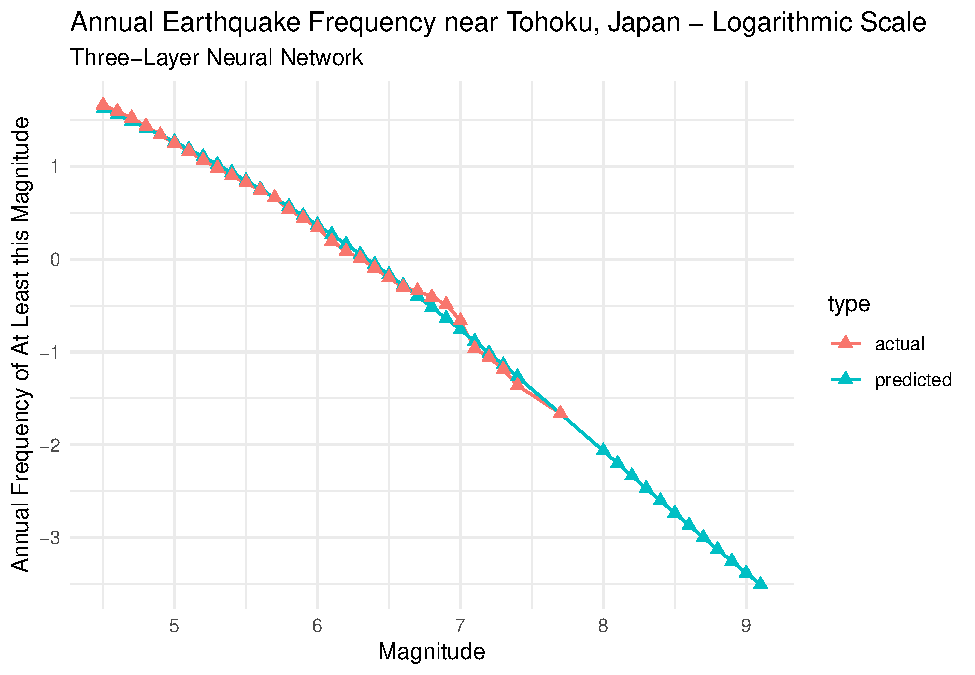
\includegraphics{earthquakes_files/figure-latex/unnamed-chunk-7-1.pdf}

\hypertarget{testing-capacity-levels-and-mse-measurements}{%
\subsection{testing capacity levels and MSE
measurements}\label{testing-capacity-levels-and-mse-measurements}}

\begin{Shaded}
\begin{Highlighting}[]
\FunctionTok{set.seed}\NormalTok{(}\DecValTok{4723}\NormalTok{)}
\CommentTok{\#{-}{-}{-}one hidden layer{-}{-}{-}}
\NormalTok{mlp }\OtherTok{\textless{}{-}} \FunctionTok{neuralnet}\NormalTok{(freqc }\SpecialCharTok{\textasciitilde{}}\NormalTok{ mag,}
                 \AttributeTok{stepmax =} \FloatTok{1e+06}\NormalTok{,}
                 \AttributeTok{data =}\NormalTok{ train,}
                 \AttributeTok{hidden =} \FunctionTok{c}\NormalTok{(}\DecValTok{5}\NormalTok{))}

\CommentTok{\#predictions on test data}
\NormalTok{pps }\OtherTok{\textless{}{-}} \FunctionTok{predict}\NormalTok{(mlp, }\AttributeTok{newdata =} \FunctionTok{data.frame}\NormalTok{(}\AttributeTok{mag =}\NormalTok{ test}\SpecialCharTok{$}\NormalTok{mag))}

\CommentTok{\#SSE to get test error}
\NormalTok{SSE1 }\OtherTok{\textless{}{-}} \FunctionTok{sum}\NormalTok{((pps }\SpecialCharTok{{-}}\NormalTok{ test}\SpecialCharTok{$}\NormalTok{freqc)}\SpecialCharTok{\^{}}\DecValTok{2}\NormalTok{)}

\FunctionTok{set.seed}\NormalTok{(}\DecValTok{4723}\NormalTok{)}
\CommentTok{\#{-}{-}{-}two hidden layers{-}{-}{-}}
\NormalTok{mlp }\OtherTok{\textless{}{-}} \FunctionTok{neuralnet}\NormalTok{(freqc }\SpecialCharTok{\textasciitilde{}}\NormalTok{ mag,}
                 \AttributeTok{stepmax =} \FloatTok{1e+06}\NormalTok{,}
                 \AttributeTok{data =}\NormalTok{ train,}
                 \AttributeTok{hidden =} \FunctionTok{c}\NormalTok{(}\DecValTok{5}\NormalTok{,}\DecValTok{5}\NormalTok{))}

\CommentTok{\#predictions on test data}
\NormalTok{pps }\OtherTok{\textless{}{-}} \FunctionTok{predict}\NormalTok{(mlp, }\AttributeTok{newdata =} \FunctionTok{data.frame}\NormalTok{(}\AttributeTok{mag =}\NormalTok{ test}\SpecialCharTok{$}\NormalTok{mag))}

\CommentTok{\#SSE to get test error}
\NormalTok{SSE2 }\OtherTok{\textless{}{-}} \FunctionTok{sum}\NormalTok{((pps }\SpecialCharTok{{-}}\NormalTok{ test}\SpecialCharTok{$}\NormalTok{freqc)}\SpecialCharTok{\^{}}\DecValTok{2}\NormalTok{)}

\FunctionTok{set.seed}\NormalTok{(}\DecValTok{4723}\NormalTok{)}
\CommentTok{\#{-}{-}{-}three hidden layers{-}{-}{-}}
\NormalTok{mlp }\OtherTok{\textless{}{-}} \FunctionTok{neuralnet}\NormalTok{(freqc }\SpecialCharTok{\textasciitilde{}}\NormalTok{ mag,}
                 \AttributeTok{stepmax =} \FloatTok{1e+06}\NormalTok{,}
                 \AttributeTok{data =}\NormalTok{ train,}
                 \AttributeTok{hidden =} \FunctionTok{c}\NormalTok{(}\DecValTok{5}\NormalTok{,}\DecValTok{5}\NormalTok{,}\DecValTok{5}\NormalTok{))}

\CommentTok{\#predictions on test data}
\NormalTok{pps }\OtherTok{\textless{}{-}} \FunctionTok{predict}\NormalTok{(mlp, }\AttributeTok{newdata =} \FunctionTok{data.frame}\NormalTok{(}\AttributeTok{mag =}\NormalTok{ test}\SpecialCharTok{$}\NormalTok{mag))}

\CommentTok{\#MSE to get test error}
\NormalTok{SSE3 }\OtherTok{\textless{}{-}} \FunctionTok{sum}\NormalTok{((pps }\SpecialCharTok{{-}}\NormalTok{ test}\SpecialCharTok{$}\NormalTok{freqc)}\SpecialCharTok{\^{}}\DecValTok{2}\NormalTok{)}

\FunctionTok{data.frame}\NormalTok{(SSE1,SSE2,SSE3)}
\end{Highlighting}
\end{Shaded}

\begin{verbatim}
##          SSE1        SSE2       SSE3
## 1 0.009838334 0.008655795 0.01114061
\end{verbatim}

\end{document}
